\documentclass{article}
\usepackage[T2A]{fontenc}
\usepackage{epigraph}
\usepackage[english, russian]{babel} % языковой пакет
\usepackage{amsmath,amsfonts,amssymb} %математика
\usepackage{mathtools}
\usepackage[oglav,spisok,boldsect,eqwhole,figwhole,hyperref,hyperprint,remarks,greekit]{../../style/fn2kursstyle}
\usepackage[utf8]{inputenc}
\usepackage[]{tkz-euclide}
\usepackage{algpseudocode}
\usepackage{pgfplots}
\usepackage{tikz-3dplot}
\usepackage[oglav,spisok,boldsect,eqwhole,figwhole,hyperref,hyperprint,remarks,greekit]{./style/fn2kursstyle}
\usepackage{multirow}
\usepackage{supertabular}
\usepackage{multicol}
\usepackage{tikz}
\usepackage{pgfplots}
\usepackage{float}
\usepackage{graphicx}
\pgfplotsset{compat=1.9}
\usepackage[svgnames]{pstricks}
\usepackage{pst-solides3d} 
\usepackage{multirow}
\usepackage{hhline}
\usepackage{slashbox}
\usepackage{pdflscape}
\usepackage{array} 
\graphicspath{{../../style/}{../}{../lab10/lab10}}

  


\newcommand{\cond}{\mathop{\mathrm{cond}}\nolimits}
\newcommand{\rank}{\mathop{\mathrm{rank}}\nolimits}
% Переопределение команды \vec, чтобы векторы печатались полужирным курсивом
\renewcommand{\vec}[1]{\text{\mathversion{bold}${#1}$}}%{\bi{#1}}
\newcommand\thh[1]{\text{\mathversion{bold}${#1}$}}
%Переопределение команды нумерации перечней: точки заменяются на скобки
\renewcommand{\labelenumi}{\theenumi)}
\newtheorem{theorem}{Теорема}
\newtheorem{define}{Определение}
\tdplotsetmaincoords{60}{115}
\pgfplotsset{compat=newest}

\title{Методы численного решения
интегральных уравнений}
\author{Н.\,О.~Акиньшин}
\group{ФН2-61Б}
\date{2025}
\supervisor{А.\,С.~Джагарян}



\begin{document}
    \maketitle
    \newpage
    \tableofcontents
    \newpage

    \section{Контрольные вопросы}
	\begin{enumerate}
		\item При выполнении каких условий интегральное уравнение
		Фредгольма 2-го рода имеет решение? В каком случае
		решение является единственным?
		\newline
		{\bfseries Ответ. } 
		Если $K(x, s)$ и $f(x)$ являются кусочно-непрерывными или удовлетворяют 
		\begin{gather*}
			\int_{a}^{b} \int_{a}^{b} |K(x, s)|^2 dx ds < \infty
			\int_{a}^{b}|f(x)|^2 dx < \infty
		\end{gather*}
		и ядро $K(x, s)$ вещественно и симметрично, то существует 
		хотя бы одна собственная функция соответствующей задачи Штурма-Лиувилля для 
		некоторого собственного значения, при этом если $\lambda$ из 
		определения интегрального уравнения Фредгольма 2-го рода 
		\begin{equation*}
			u(x) - \lambda \int_{a}^{b}K(x,s)u(s)ds = f(x)
		\end{equation*}
		не равно собственному значению задачи Штурма-Лиувилля, то уравнение имеет единственное решение.
		\item Можно ли привести матрицу СЛАУ, получающуюся при
		использовании метода квадратур, к симметричному виду
		в случае, если ядро интегрального уравнения является
		симметричным, т. е. $K(x, s) = K(s, x)$?
		\newline
		{\bfseries Ответ. } 
При использовании метода квадратур требуется решать систему уравнений вида
	
	
	\[
	y_i - \lambda \sum_{k=0}^{N} a_k^N K(x_i, s_k) y_k = f(x_i)
	\]
	Используем формулу трапеций, тогда матрица системы имеет вид
	\[
	\begin{pmatrix}
		1-\frac{\lambda h}{2} K(x_0, s_0) & -\lambda h K(x_0, s_1) & -\lambda h K(x_0, s_2) & \cdots & -\frac{\lambda h}{2} K(x_0, s_N) \\
		-\frac{\lambda h}{2} K(x_1, s_0) & 1-\lambda h K(x_1, s_1) & -\lambda h K(x_1, s_2) & \cdots & -\frac{\lambda h}{2} K(x_1, s_N) \\
		\vdots & \vdots & \vdots & \ddots & \vdots \\
		-\frac{\lambda h}{2} K(x_N, s_0) & -\lambda h K(x_N, s_1) & -\lambda h K(x_N, s_2) & \cdots & 1-\frac{\lambda h}{2} K(x_N, s_N) \\
	\end{pmatrix}
	\]

	Из матрицы видно, что даже при симметрии ядра $K$ симметрия матрицы достигаться не будет т.к. есть множитель 1/2. Например $a_12 \neq a_21$
		\item Предложите способ контроля точности результата вычислений при использовании метода квадратур.
		\newline
		{\bfseries Ответ. } 
		Пусть есть численное решения $I_h$, которое получено методом квадратур
		порядка $p$, 
		тогда погрешность на сетке $\Omega_h$ $z_h$ можно представить в виде
		\begin{equation*}
			z_h = O(h^p) = C h^p
		\end{equation*}  
		При этом при уменьшении шага сетки получим 
		\begin{equation*}
			z_{h/2} = O((h/2)^p) = C (h/2)^p 
		\end{equation*}
		Т.к. $z_h = I^* - I_h$ и $z_{h/2} = I^* - I_{h/2}$, 
		то вычитая одно из другого получим 
		\begin{equation*}
			I_h - I_{h/2} = C h^p (1 - \frac{1}{2^p})
		\end{equation*}
		Тогда точность на сетке $\Omega_h$ будет 
		равна 
		\begin{equation*}
			z_h = \frac{I_h - I_{h/2}}{(1 - \frac{1}{2^p})}
		\end{equation*}
		\item Оцените возможность и эффективность применения методов квадратур, простой итерации и замены ядра при
		решении интегральных уравнений Вольтерры 2-го рода
		\newline
		{\bfseries Ответ. } 
		Интегральное уравнение Вольтерра 2-ро рода
	\[
	u(x) - \lambda \int_{a}^{x} K(x,s)u(s)ds = f(x)
	\]
	
	
	1. Метод квадратур
	
	
	Получим систему 
	\[
	y_i - \lambda \sum_{k=0}^{i} a_k^N K(x_i, s_k) y_k = f(x_i)
	\]
	
	\[
	\begin{pmatrix}
		1 & 0 &0 & 0 & ... & 0 \\
		-\frac{\lambda h}{2} K(x_1, s_0) & 1 - \frac{\lambda h}{2} K(x_1, s_1) & 0 & 0 & ... & 0\\
		-\frac{\lambda h}{2} K(x_2, s_0) & -\lambda h K(x_2, s_1) & 1-\frac{\lambda h}{2} K(x_2, s_2) &0 & ... & 0 \\
		-\frac{\lambda h}{2} K(x_3, s_0) & -\lambda h K(x_3, s_1) & -\lambda h K(x_3, s_2) & 1 - \frac{\lambda h}{2} K(x_3, s_3) & ... & 0\\
		-\frac{\lambda h}{2} K(x_N, s_0) & -\lambda h K(x_N, s_1) & -\lambda h K(x_N, s_2) & -\lambda h K(x_N, s_2)&\cdots & 1-\frac{\lambda h}{2} K(x_N, s_N) 
	\end{pmatrix}
	\]
	
	
	Матрица в отличии от Фрдегольма 2ро рода является нижне треугольной, что облегчает решение СЛАУ. Можно воспользоваться обратным ходом Гаусса и получить $O(n^2)$ операций где $n$ -- количество узлов в сетке.
	
	
	2. Метод Простой итерации
	
	 
	Можно реализовать аналогично уравнению Фредгольма 2ро рода 
	
	
	\[
	u^{(k+1)}(x) = f(x) + \lambda \int_{a}^{x}K(x,s) u^{(k)}(s)ds
	\]
	
	Для перехода на следующую итерацию потребуется вычислять интеграл. Используем формулу трапеций. В уравнении Фредгольма 2-ро рода требуется $2n*n = 2n^2$ операций для перехода на следующую итерацию. В уравнении Вольтерра 2-ро рода потребуется 
	\[
	\sum_{i=0}^{n}2i = n(1 + n)
	\]
	что меньше чем в уравнении Фредгольма 2ро рода
	
	
	3. с вырожденным ядром
	
	
	\[
	K(x,s) = \sum_{i=1}^{m} \phi_i(x) \psi(s)
	\]
	Подставим представление в уравнение Вольтерра 2-ро рода
	
	\[
	u(x) - \lambda \sum_{i=1}^{m} \phi_i(x) \cdot \int_{a}^{x} \psi_i(s) u(s)ds = f(x)
	\]
	
	Введем обозначения
	\[
	\int_{a}^{x} \psi_i(s) u(s)ds = C_i(x)
	\]
	Тогда решение представляется в виде
	\[
	u(x) =  \lambda \sum_{i=1}^{m} \phi_i(x)C_i(x) +f(x)
	\]
	
	Требуется найти функции $C_i(x)$
	
	
	Подставляя данное представление в исходное уравнение получаем
	
	\[
	\sum_{i=1}^{m}[C_i(x) - \int_{a}^{x} \psi_i(s)(f(s) + \lambda \sum_{j=1}^{m}C_j(x)\phi_j(s))ds] \phi_i(x) =0
	\]
	Далее в случаи Фредгольма 2ро рода получалось воспользоваться независимостью функции $\psi_i(x)$, однако здесь так не получиться поскольку коэффициенты являются функции зависящие от $x$. Поэтому метод разделения ядер не применим в случае уравнение Вольтерра 2-ро рода

		\item Что называют резольвентой ядра интегрального уравнения?
		\newline 
		{\bfseries Ответ. } 
		Рассмотрим интегральное уравнение 
		\begin{equation*}
			u(x) - \lambda \int_{a}^{b} K(x, s) u(s)ds = f(x)
		\end{equation*}
		Для его ядра $K(x,s)$ резольвентой называют такую функцию $R(x, s, \lambda)$:
		\begin{equation*}
			u(x)= f(x) + \lambda \int_{a}^{b} R(x, s, \lambda) f(s)ds
		\end{equation*} 
		\item Почему замену ядра интегрального уравнения вырожденным предпочтительнее осуществлять путем разложения по
		многочленам Чебышева, а не по формуле Тейлора?
		\newline 
		{\bfseries Ответ. } 
		\newline
		1.Многочлены Чебышева минимизируют погрешность на всем отрезке сходимости, в отличии от Формулы Тейлора, которая гарантирует сходимость лишь в окрестности раскладываемой точки т.е. Формула Тейлора является своего рода экстраполяцией нашей функции, а экстраполяция обладает плохими свойствами. В отличии от разложение Чебышева.
		\newline
		2.При разложении в формулу Тейлора могут возникать осциляции на концах отрезка. Чебышевское же приближение избегает такого эффекта.
		\item Какие вы можете предложить методы решения переопределенной системы (5.13), (5.17) помимо введения дополнительно переменной R?
		\newline 
		{\bfseries Ответ. } 
		Получается переопределенная система
		\begin{equation*}
			\begin{cases}
				\mathbf{n} \cdot  \sum_{j=1}^N \mathbf{Q}(\mathbf{k_i}, \mathbf{c_j}) g_j \Delta l_j = f(\mathbf{k_i}) \\ 
				\sum_{j=1}^{N} g_j \Delta l_j = 0
			\end{cases}
		\end{equation*}
		В силу того, что число неизвестных меньше, чем число уравнений, то не существует решения, 
		которое удовлетворяло бы этой системе, при условии, что её ранг равен $N+1$.
		Тогда решение этой системы можно приблизить, например, с помощью метода наименьших 
		квадратов. 
		Обозначим матрицу коэффициентов системы за $A$, $\mathbf{b}$ - вектор правой части
		Тогда будем искать решение следующей задачи поиска безусловного минимума 
		\begin{equation*}
			(A \mathbf{g} - \mathbf{b})^T (A \mathbf{g} - \mathbf{b})\to \min\limits_{\mathbf{g} \in \mathbb{R}^{N}}
		\end{equation*}
		То есть происходит поиск такого приближения $\mathbf{g}$, что 
		данное приближение удовлетворяет условия минимума сумме квадратов отклонений.
		Известно, что решение такой задачи можно найти аналитически 
		\begin{equation*}
			\mathbf{g} = (A^T A )^{-1}A^T \mathbf{g	}
		\end{equation*}
	\end{enumerate}
	\section{Порядки}
		\begin{table}[H]
		\centering
		\caption{Порядок аппроксимации для метода квадратур с использованием метода трапеций}
		\begin{tabular}{|c|c|}
			\hline
			Количество точек & Порядок \\ \hline
			10 &1.99782\\ \hline
			20 &1.99945\\ \hline
			40 &1.99986\\ \hline
			80 &1.99997\\ \hline
			160 &1.99999\\ \hline
		\end{tabular}
	\end{table}

			\begin{table}[H]
		\centering
		\caption{Зависимость погрешности от количества членов разложения}
		\begin{tabular}{|c|c|}
			\hline
			Кол-во членов разл. & Погрешность \\ \hline
			2 &0.148054\\ \hline
			3 &0.0440627\\ \hline
			4 &0.0105949\\ \hline
			5 &0.00208607\\ \hline
			6 &0.000344697\\ \hline
			7 &4.89523e-05\\ \hline
			8 &6.09131e-06\\ \hline
			9 &6.73798e-07\\ \hline
			10 &6.65161e-08\\ \hline
			11 &5.35044e-09\\ \hline
			12 &6.04542e-10\\ \hline
		\end{tabular}
	\end{table}

				\begin{table}[H]
		\centering
		\caption{Зависимость погрешности от количества итераций}
		\begin{tabular}{|c|c|}
			\hline
			Кол-во итераций & Погрешность \\ \hline
			1 & 0.110833\\ \hline
			2 & 0.036574\\ \hline
			3 & 0.0117899\\ \hline
			4 & 0.00351821\\ \hline
			5 & 0.000757536\\ \hline
			6 & 0.000163839\\ \hline
			7 & 0.000471348\\ \hline
			8 & 0.000573979\\ \hline
			9 & 0.000608232\\ \hline
			10 & 0.000619664\\ \hline
			11 & 0.00062348\\ \hline
			12 & 0.000624753\\ \hline
			13 & 0.000625178\\ \hline
			14 & 0.00062532\\ \hline
			15 & 0.000625367\\ \hline
			16 & 0.000625383\\ \hline
			17 & 0.000625388\\ \hline
			18 & 0.00062539\\ \hline
			19 & 0.000625391\\ \hline
			20 & 0.000625391\\ \hline
		\end{tabular}
	\end{table}
	\begin{figure}[H]
        \centering
        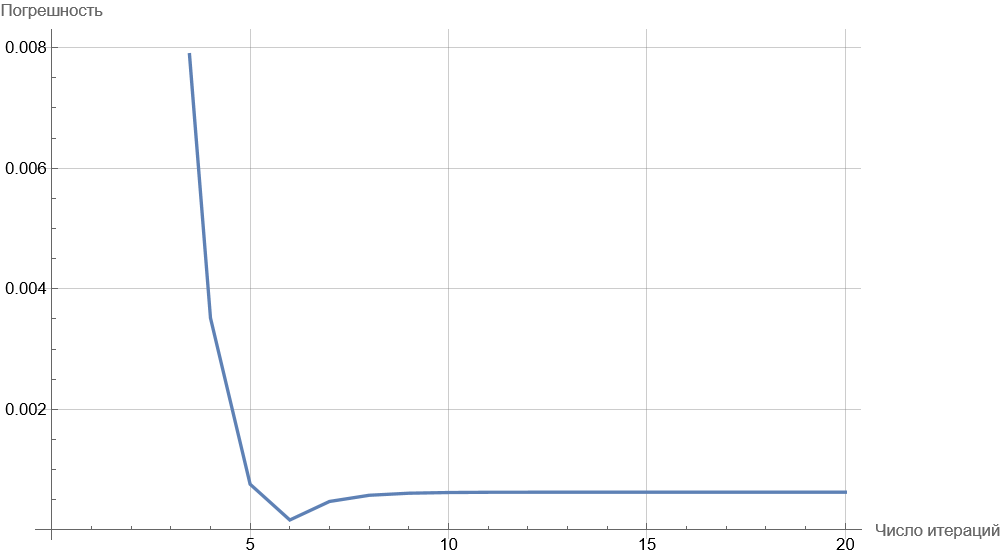
\includegraphics[width=\textwidth]{iterationImage.png}
        \caption{Зависимость погрешности от числа итерация для метода простой итерации}
    \end{figure}
	\section{Результаты}

	\begin{figure}[H]
        \centering
        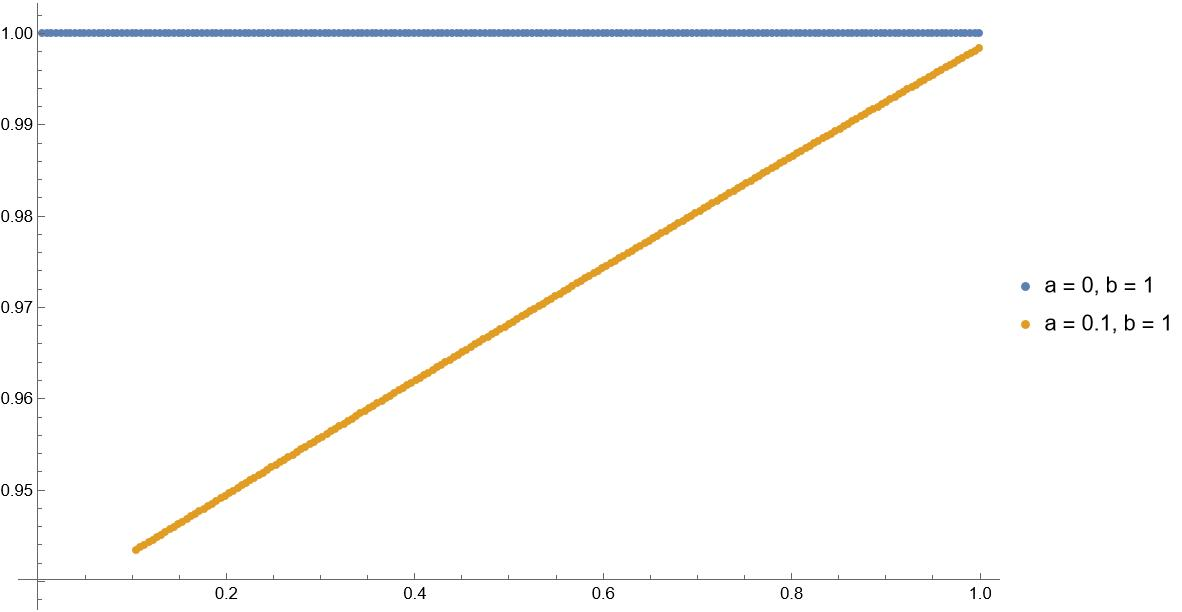
\includegraphics[width=\textwidth]{test1_SIM.jpg}
        \caption{Пример 1 для метода простой итерации}
    \end{figure}
		\begin{figure}[H]
        \centering
        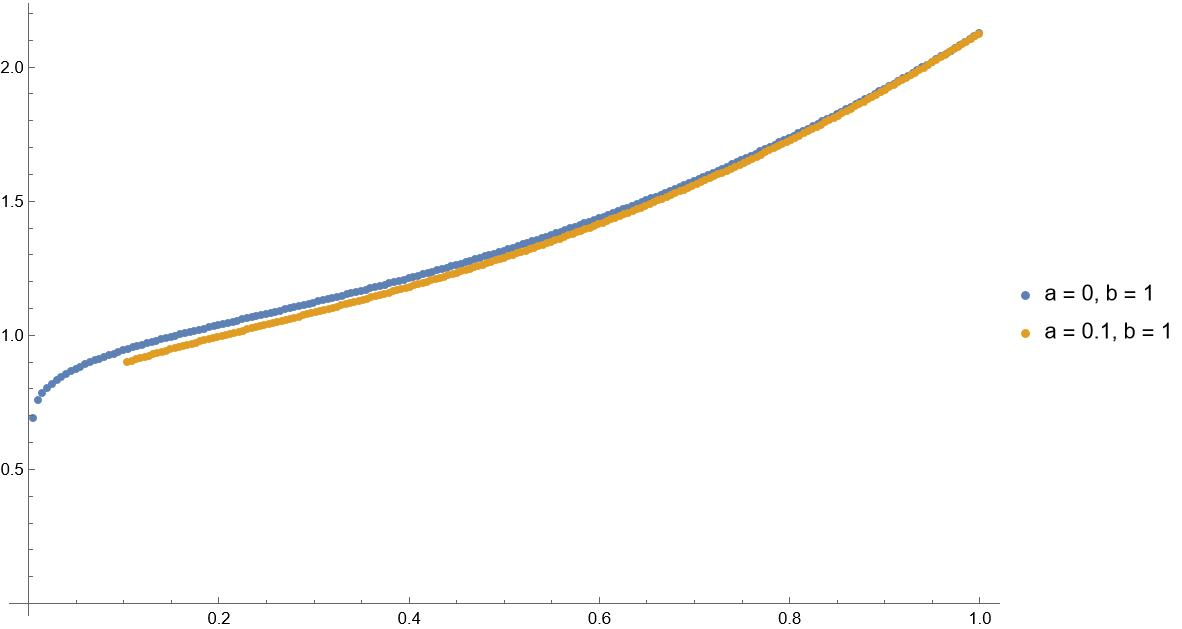
\includegraphics[width=\textwidth]{test2_SIM.jpg}
        \caption{Пример 2 для метода простой итерации}
    \end{figure}

	\begin{figure}[H]
        \centering
        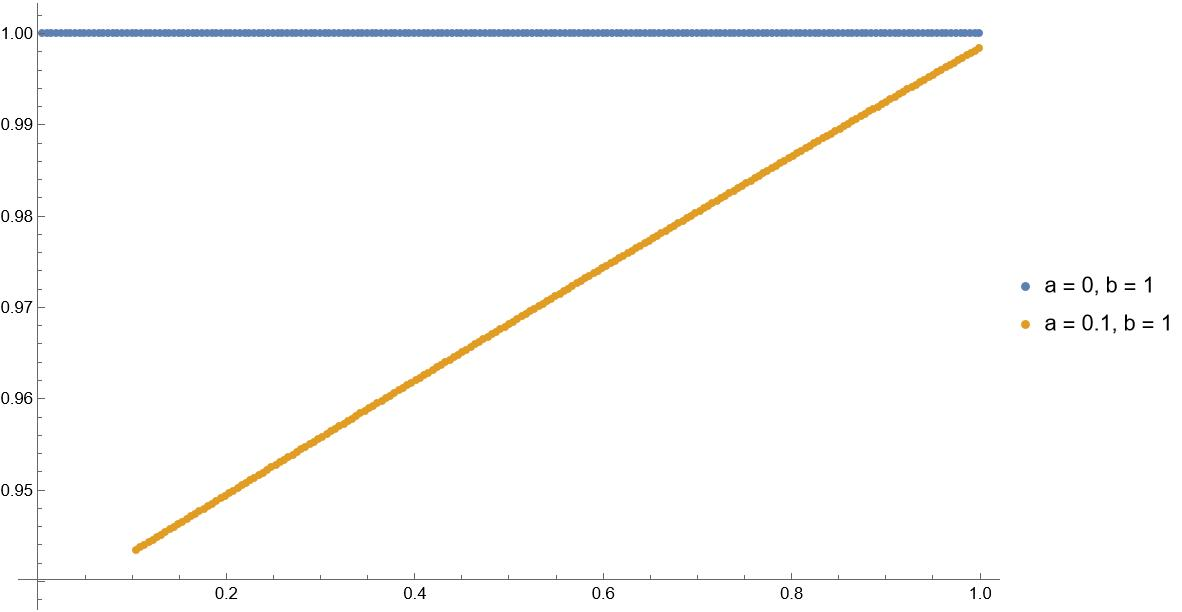
\includegraphics[width=\textwidth]{test1_kv.jpg}
        \caption{Пример 1 для метода квадратур}
    \end{figure}
		\begin{figure}[H]
        \centering
        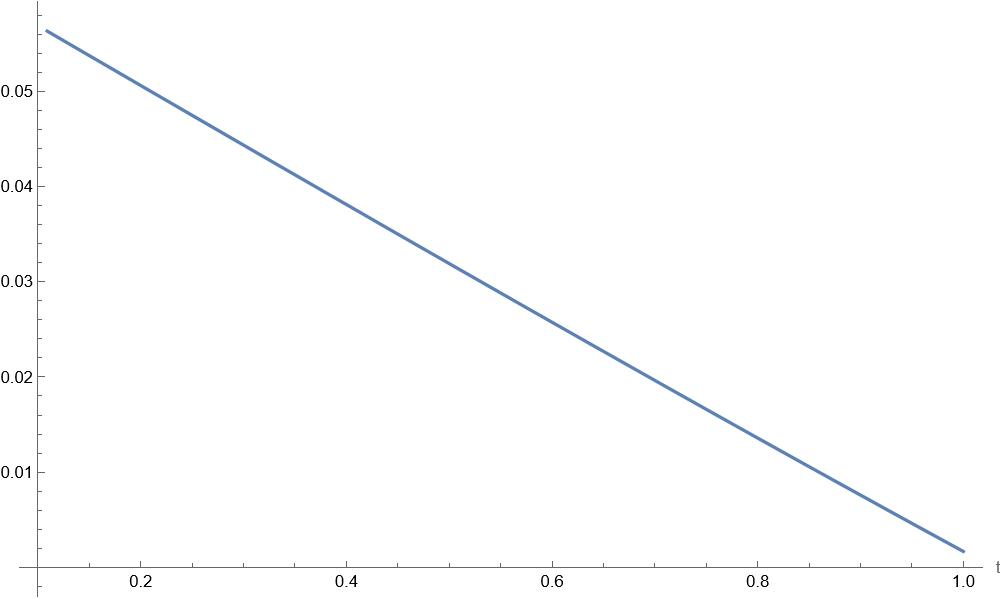
\includegraphics[width=\textwidth]{diff_test1.jpg}
        \caption{Погрешность примера 1}
    \end{figure}
		\begin{figure}[H]
        \centering
        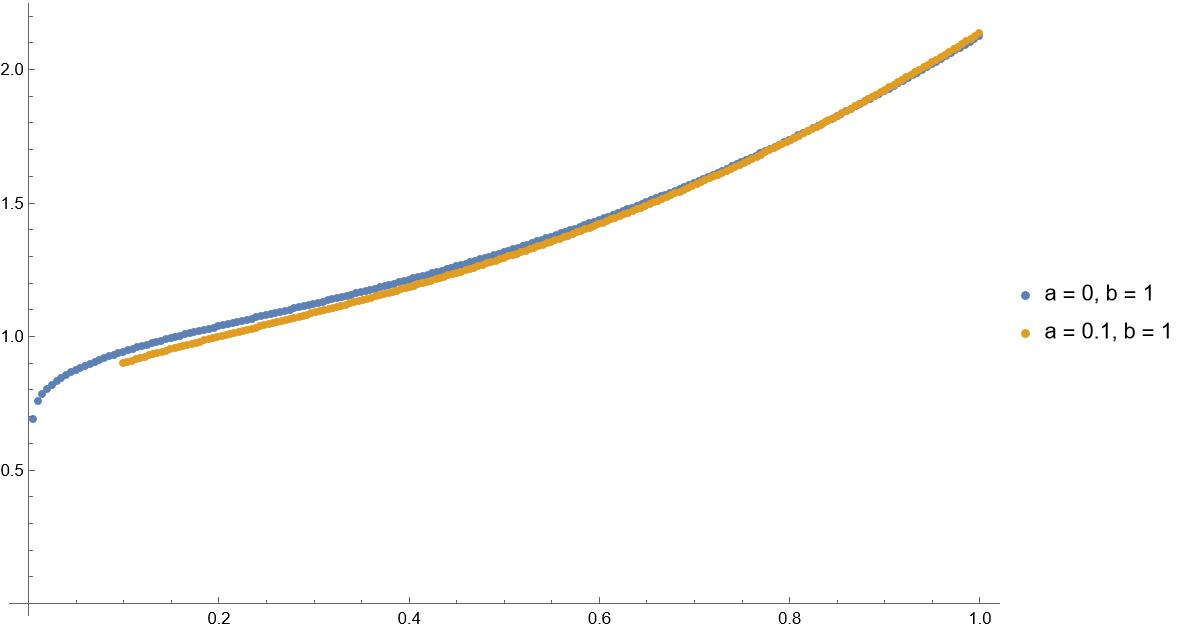
\includegraphics[width=\textwidth]{test2_kv.jpg}
        \caption{Пример 2 для метода квадратур}
    \end{figure}
			\begin{figure}[H]
        \centering
        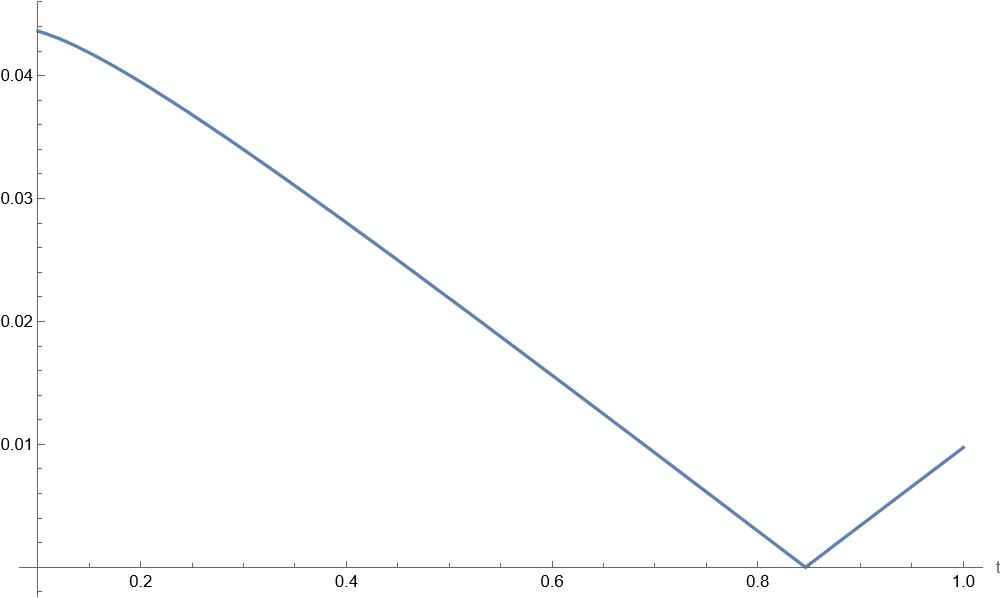
\includegraphics[width=\textwidth]{diff_test2.jpg}
        \caption{Погрешность примера 2}
    \end{figure}
	\begin{figure}[H]
        \centering
        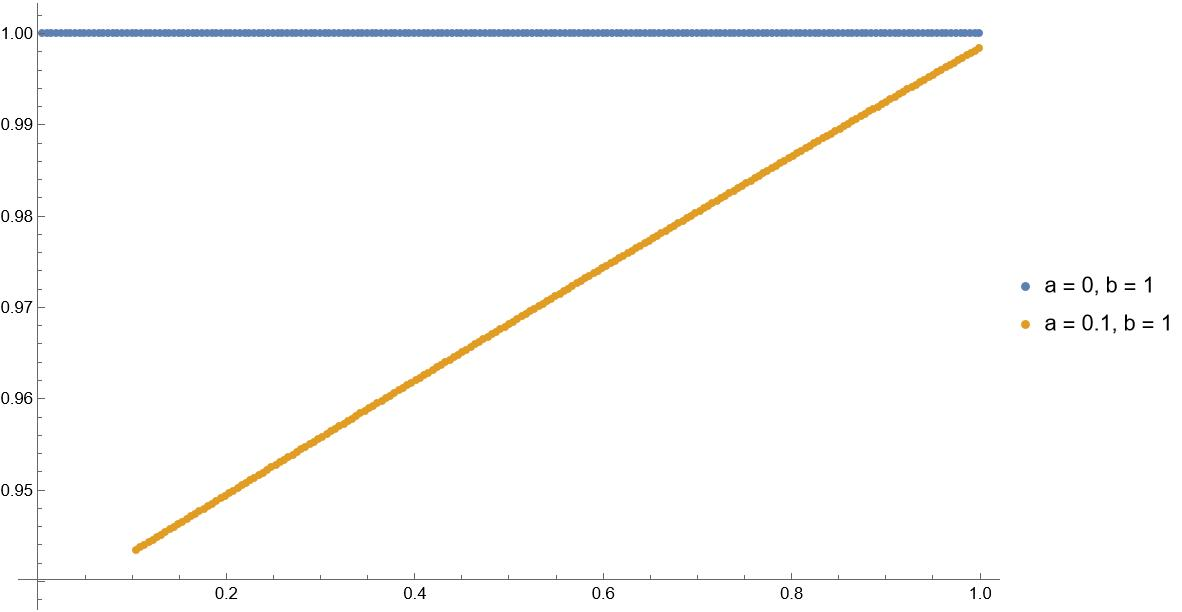
\includegraphics[width=\textwidth]{test1_kv.jpg}
        \caption{Пример 1 для метода разложения ядра}
    \end{figure}
	\begin{figure}[H]	
        \centering
        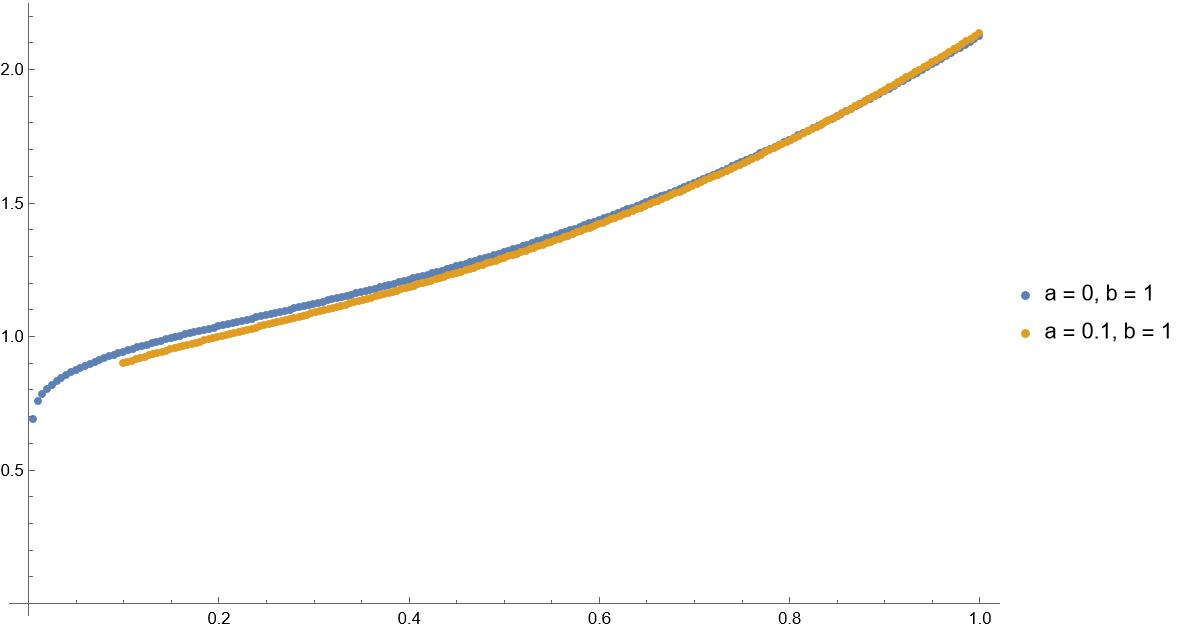
\includegraphics[width=\textwidth]{test2_kv.jpg}
        \caption{Пример 2 для метода разложения ядра}
    \end{figure}
	\begin{figure}[H]
        \centering
        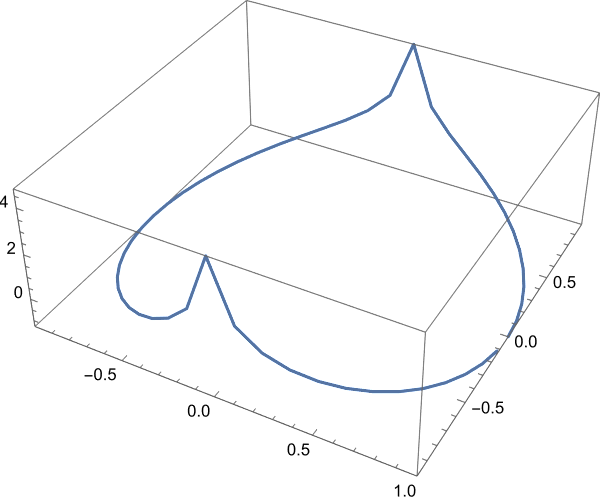
\includegraphics[width=\textwidth]{singular.png}
        \caption{Пример для сингулярного уравнения}
    \end{figure}

	\begin{figure}[H]
        \centering
        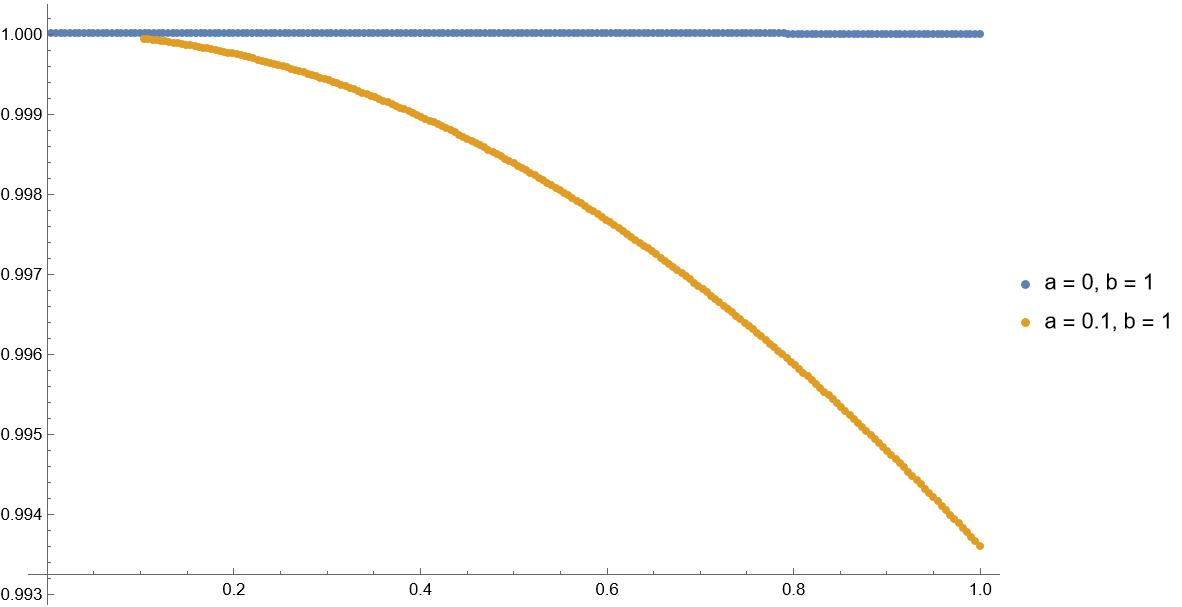
\includegraphics[width=\textwidth]{var1.jpg}
        \caption{Вариант 1. Метод квадратур, правая часть 1}
    \end{figure}
	\begin{figure}[H]
        \centering
        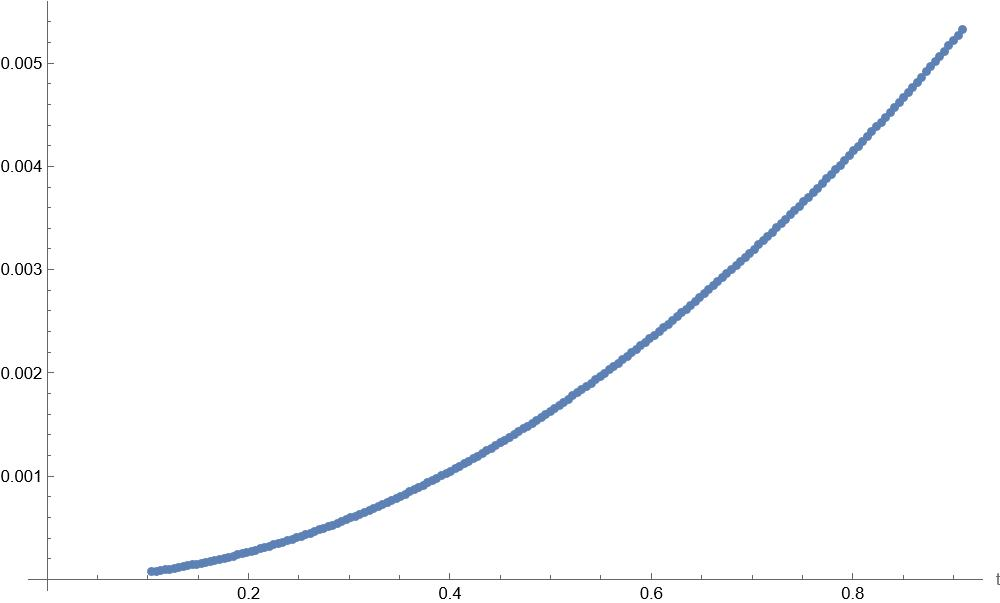
\includegraphics[width=\textwidth]{diff_var2.jpg}
        \caption{Разница решений для задания по вариантам}
    \end{figure}
	\begin{figure}[H]
        \centering
        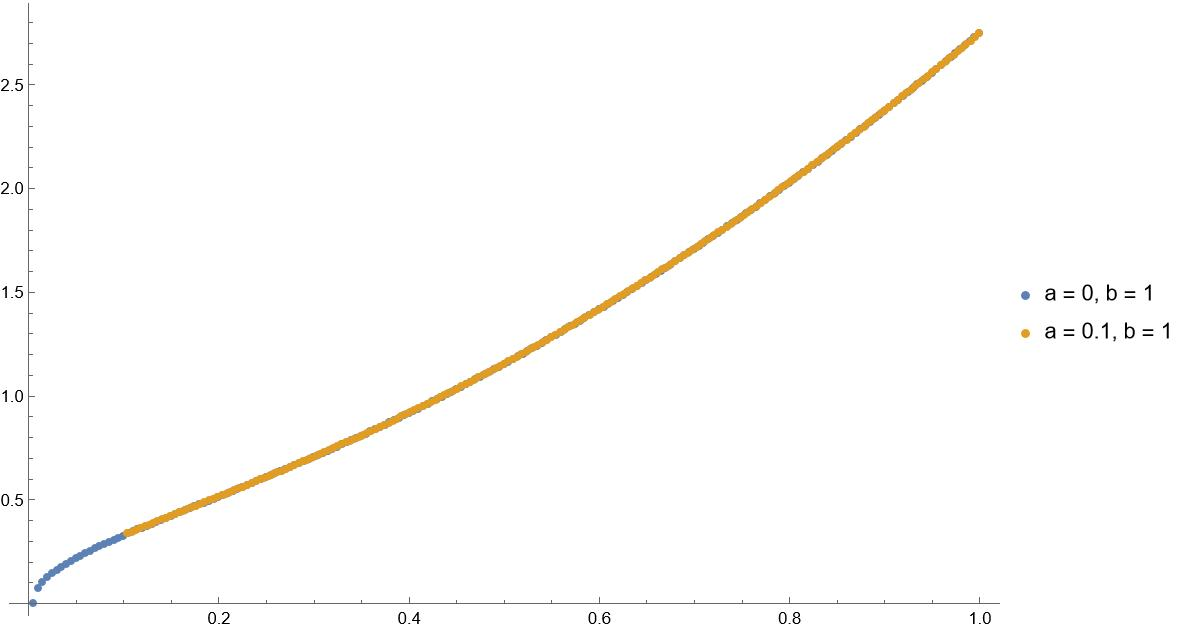
\includegraphics[width=\textwidth]{var2.jpg}
        \caption{Вариант 1. Метод квадратур, правая часть 2}
    \end{figure}
		\begin{figure}[H]
        \centering
        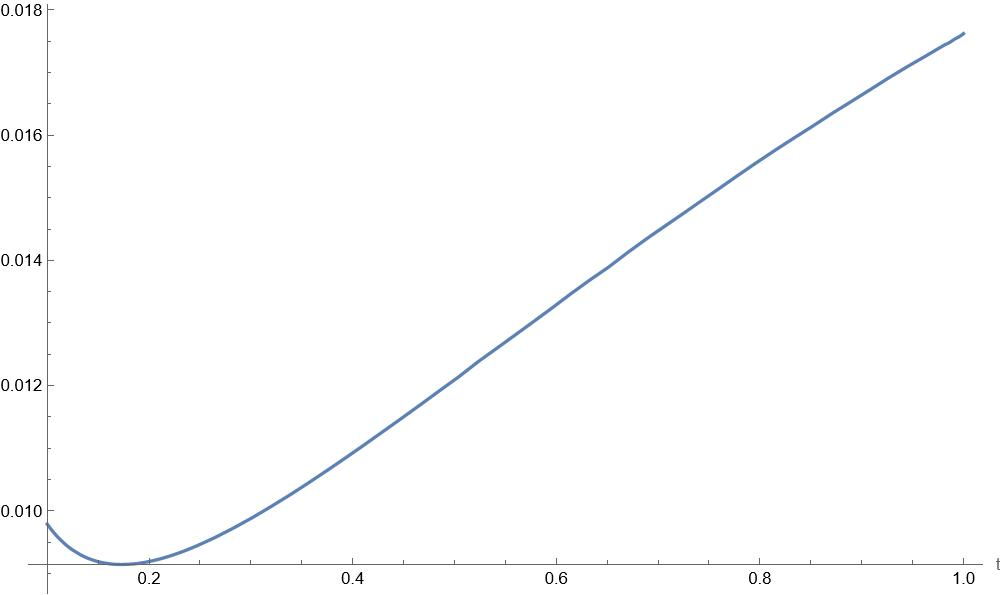
\includegraphics[width=\textwidth]{diff_var_2.jpg}
        \caption{Погрешность решения варианта 1 при правой части 2}
    \end{figure}
			\begin{figure}[H]
        \centering
        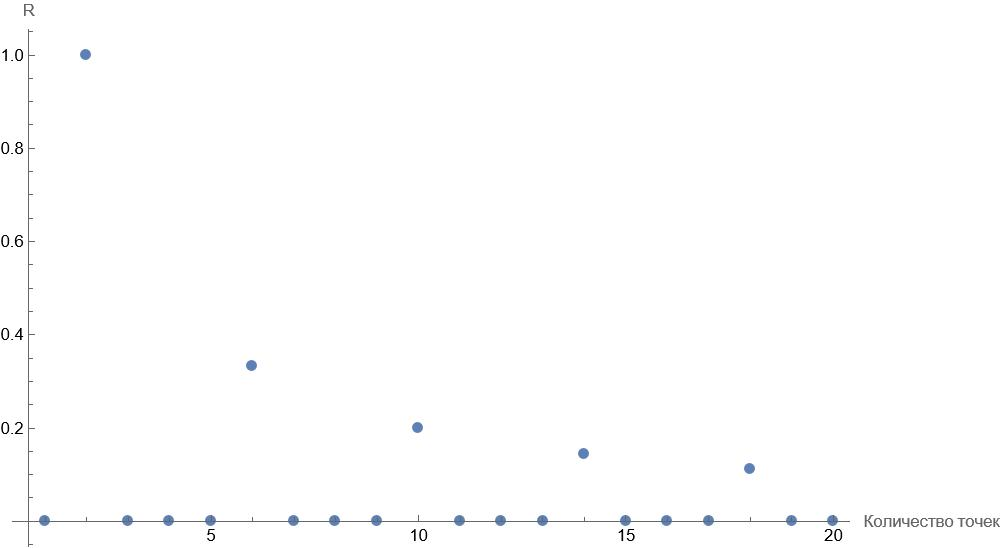
\includegraphics[width=\textwidth]{R.jpg}
        \caption{Зависимость R от числа точек на контуре }
    \end{figure}

	\section{Дополнительные вопросы}
	\begin{enumerate}
		\item Что такое альтернатива Фредгольма?
		\newline 
		{\bfseries Ответ. } 
		Для вполне непрерывного оператора $A \in \mathcal{L}(X)$, 
		где $X $-- банахово пространство, число собственных значений
		конечно либо счетно. Все собственные значения можно представить
		в виде конечной или бесконечной последовательности $\{ \lambda_n\}$,
		причем 
		\begin{equation*}
			|\lambda_1| \geqslant |\lambda_2| \geqslant \ldots \geqslant
			|\lambda_n| \geqslant ... 
		\end{equation*}
		Если последовательность бесконечна, то $\lambda_n \to 0  \text{ при } n \to \infty$.

		\item Свойства полинома Чебышева
				\newline 
		{\bfseries Ответ. } 

		Пусть $T_n(x)$ -- полином Чебышева первого рода. 
		Тогда справедливы следующие свойства
		\begin{enumerate}
			\item При четном $n$ полином $T_n$ является четной 
			функцией, а при нечетном - нечетной.
			\item Если $x \in [-1,1]$, то справедлива формула 
			\begin{equation*}
				T_n(x) = \cos (n \arccos x)
			\end{equation*}
			\item При $n \geqslant 1$ $T_n$ имеет $n$ корней 
			$x_k \in \mathbb{R}: x_k \in[-1,1] $ 
			\item Среди всех многочленов фиксированной степени $n \geqslant 1$
			 со старшим коэффициентом равным 1, наименьшее уклонение от 
			 нуля равное $2^{1-n}$ имеет 
			 многочлен $\tilde{T}_n(x) = 2^{1-n}T_n(x)$,
			 то есть справедливо 
			 \begin{equation*}
				\max\limits_{x \in [-1, 1]} |P_n(x)| = \tilde{T}_n(x)
			 \end{equation*}
		\end{enumerate}
		\item Сходимость метода простой итерации
				\newline 
		{\bfseries Ответ. } 
		1)Для уравнения Фредгольма 2-ро рода метод последовательных приближений имеет вид 
	
	\[
	u_{n+1}(x) = f(x) + \lambda \int_{a}^{b}K(x, \xi) u_n(\xi) d\xi
	\]
	
	уравнение Фредгольмо 2ро рода имеет вид 
	
	\[
	u(x) = f(x) + \lambda \int_{a}^{b}K(x, \xi) u(\xi) d\xi
	\]
	
	Вычтем одно из другого и введем погрешность
	
	
	\[
	z_{n+1}(x) = u_{n+1}(x) - u(x) = \lambda \int_{a}^{b}K(x, \xi) z_n(\xi) d\xi
	\]
	
	Тогда оценим норму
	
	\[
	||z_{n+1}(x)||_C \le  |\lambda|(b-a)||K(x, \xi)||_C ||z_n(x)||_C = q ||z_n(x)||_C
	\]
	где $q = |\lambda|(b-a)||K(x, \xi)||_C$.
	
	
	Если $q<1$, то итерации сходятся равномерно по х, причем сходимость линейная
	
	
	
	2)Для уравнение Вольтерра
	
	\[
	z_{n+1}(x) = u_{n+1}(x) - u(x) = \lambda \int_{a}^{x}K(x, \xi) z_n(\xi) d\xi
	\]
	
	\[
	z_1(x) = \lambda \int_{a}^{x}K(x, \xi) z_0(\xi) d\xi \le |\lambda| \cdot ||K(x,\xi)||_C \cdot ||z_0||_C\int_{a}^{x} d\xi = |\lambda| \cdot ||K(x,\xi)||_C ||z_0||_C(x-a)
	\]
	
	\[
	z_2(x) = \lambda \int_{a}^{x}K(x, \xi) z_1(\xi) d\xi \le (\lambda \cdot||K(x,\xi)||_C )^2||z_0||_C \int_{a}^{x}(\xi-a) d\xi = (\lambda \cdot||K(x,\xi)||_C )^2||z_0||_C \frac{(x-a)^2}{2}
	\]
	
	
	\[
	z_{n+1}(x) \le ||z_0||_C(|\lambda| \cdot||K(x,\xi)||_C )^n \cdot \frac{(x-a)^n}{n!}
	\]
	
	Тогда норма оценивается 
	\[
	||z_{n+1}(x)||_C \le (|\lambda| \cdot||K(x,\xi)||_C )^n \cdot \frac{(b-a)^n}{n!}||z_0||_C
	\]
	
	Тогда метод сходится равномерно по $\lambda$ и по $х$ , если $q = |\lambda| \cdot||K(x,\xi)||_C<1$. за счет факториала
		\item Как получить симметричную матрицу?
		\newline
		{\bfseries Ответ. } 
		\[
	u(x) - \lambda \int_{a}^{b}K(x,s)u(s)ds = f(x)
	\]
	Дробим интеграл на куски и получаем
	\[
	u(x) - \lambda \sum_{k=0}^{N-1} \int_{s_k}^{s_{k+1}} K(x,s)u(s)ds = f(x)
	\]
	
	
	Аппроксимируем интеграл формулой левых прямоугольников 
	\[
	\int_{x_i}^{x_{i+1}} K(x,s)u(s)ds = K(x, s_k) u(s_k) h
	\]
	
	Получаем СЛАУ
	\[
	y_i - \lambda \sum_{k=0}^{N-1} K(x_i, s_k) y_k h = f(x_i)
	\]
	Матрица данной СЛАУ имеет вид
	\[
	\begin{pmatrix}
		1-\lambda hK(x_0, s_0) & -\lambda h K(x_0, s_1) & -\lambda h K(x_0, s_2) & \cdots & 0 \\
		-\lambda h K(x_1, s_0) & 1-\lambda h K(x_1, s_1) & -\lambda h K(x_1, s_2) & \cdots & 0 \\
		\vdots & \vdots & \vdots & \ddots & \vdots \\
		-\lambda h K(x_N, s_0) & -\lambda h K(x_N, s_1) & -\lambda h K(x_N, s_2) & \cdots & 1 \\
	\end{pmatrix}
	\]
	
	
	Видно, что при помощи левых либо правых прямоугольников получается не симметричная матрица.
	
	
	Однако можно последнее уравнение при $i = N$ аппроксимировать на всем отрезке правым прямоугольником
	
	т.е. 
	
	
	\[
	u(x_N) - \lambda K(x_N, s_N) u(x_N)(b-a) = f(x_N)
	\]
	
	\[
	y_N - \lambda K(x_N, s_N) y_N (b-a) = f(x_N)
	\]
	
	Тогда матрица СЛАУ будет иметь вид 
	
	\[
	\begin{pmatrix}
		1-\lambda hK(x_0, s_0) & -\lambda h K(x_0, s_1) & -\lambda h K(x_0, s_2) & \cdots & 0 \\
		-\lambda h K(x_1, s_0) & 1-\lambda h K(x_1, s_1) & -\lambda h K(x_1, s_2) & \cdots & 0 \\
		\vdots & \vdots & \vdots & \ddots & \vdots \\
		0 & 0 & 0 & \cdots & 1 -\lambda K(x_N, s_N) (b-a)\\
	\end{pmatrix}
	\]
	
	
	Тогда матрица при симметричном ядре будет симметричной. 
	\end{enumerate}
\end{document}
